\label{chapter:related-work}
\chapter{Related Work}

\section{Distributed Storage Systems}

Distributed storage comes in two flavors --- centralized and decentralized.
Centralized systems are mostly proprietary and are either used by companies or are offered as a service.
Decentralized systems are mostly open-source and are used by academia, individuals, and occasionally companies.

There are many decentralized storage systems that have been developed over the years.
While there exist decentralized networks, which are focusing on decentralized computing,
most of the decentralized networks are used for storage or some form of data sharing.
There are different kinds of decentralized storage:
\begin{enumerate}
    \item \textbf{Unstructured networks} --- nodes are connected to each other without any specific topology.
    \item \textbf{Decentralized Hash Tables} --- key-value store where the keys are distributed among the nodes.
    \item \textbf{Blockchain based storage} --- data is stored in a blockchain, or cryptocurrency
        is rewarded to users who share their available storage.
\end{enumerate}

We will mainly focus on decentralized hash tables, as they are the most popular and are used by
most of the decentralized storage systems.
Unstructured networks are used for general purpose storage, but are not as efficient as 
Blockchain based storage is niche and is not used for general purpose storage.
There are many ways to categorize networks, and we will cover some of them here.

\begin{enumerate}
    \item \textbf{Structured/Unstructured} --- Networks can have a predefined topology,
        or they can be constructed at random.
        A downside of unstructured networks is often the discovery of resources.
        Since a resource can be at any node,
        typically such networks broadcast queries through the whole network.
        This is both inefficient and can also cause traffic congestion.
        In modern structured networks the query time is $O(\log n)$,
        where $n$ is the number of nodes in the network.
    \item \textbf{Keyspace} --- the size of the keyspace can vary between different networks.
        Most networks use a keyspace of the form $2^b$, where $b$ is the number of bits.
        Each node in the network is assigned a peer ID, which is a random number in the keyspace.
        A good distribution of the peer IDs is important for the performance of the network,
        therefore the peer IDs are usually generated using a cryptographic hash function such as SHA-256.
    \item \textbf{Naming Scheme} --- how the files are named in the network.
        When storing files, an ID is generated for the file, which determines its location in the network.
        Usually the name of the file or the contents of the file are hashed to produce the key.
        More rarely, the key of the file is chosen by the user.
        While this allows for human-friendly names,
        it has a downside that it could be subject to dictionary attacks.
    \item \textbf{Replication} --- if and how the data is replicated in the network.
        Replication usually works by storing the file on the $k$ closest nodes to the key of the file.
        More rarely replication is only achieved by caching the file at different nodes.
    \item \textbf{Anonymity} --- some networks are designed to provide anonymity to the users.
        Anonymity means that the identity of the user, the data they are storing or requesting,
        the queries, and the location of the data are hidden.
        Networks usually achieve this by using onion routing and cover traffic.
        Additionally, the network caches the files aggressively,
        so the original storage node is hard to trace.
        Anonymity usually means that the network cannot provide any guarantees about
        the integrity of the data, as it should not be possible to be traced.
    \item \textbf{Security} --- what security guarantees the network provides
        Security is a major concern in decentralized networks because
        the network is open to anyone, and there is no central authority to enforce rules,
        in contrast to centralized storage systems.
        Peers can join and leave the network at any time, and they can lie about their identity and the data they store.
        We call such peers malicious.

        When we talk about security we assume that the underlying physical connection provides no security guarantees.
        Attackers can eavesdrop on the communication between nodes, modify the messages, and even drop them.
        They can also spoof IP addresses and there is no authentication of data packets in the underlying network.
        This is a reasonable assumption as most decentralized networks are built on top of the Internet,
        which is inherently insecure.

        Security can be defined as the ability of the network to detect and prevent attacks.
        S/Kademlia \cite{skademlia} summarizes the main attacks on decentralized networks:
        \begin{enumerate}
            \item \textbf{Eclipse attacks} --- an attacker isolates a node from the rest of the network.
            \item \textbf{Sybil attacks} --- a single entity pretends to be multiple entities.
            \item \textbf{Churn attacks} --- an attacker joins and leaves the network repeatedly.
            \item \textbf{Adversarial routing} --- an attacker returns adversarial routing information.
            \item \textbf{Denial-of-service attacks} --- an attacker floods the network with requests.
            \item \textbf{Storage attacks} --- an attacker manipulates the data stored on a node.
        \end{enumerate}
    \item \textbf{Persistence} --- how long the data is stored in the network.
        One of the possible approaches is to let a file be available as long as there is interest in it,
        i.e., it is being requested.
        This can be expanded in a way that rare files or rare pieces are more valuable and
        networks that employ a bartering system can use this to incentivize peers to store them.
        Another approach is to republish the file every $X$ amount of time,
        e.g., every 1 hour, to ensure that the file is still available.
        Networks that use this mechanism also use it to ensure that the data is stored on
        the correct nodes, in case a node goes offline, or a new, closer node, joins the network.
        Additionally, some networks split the files into chunks and replicate them separately.
        The most reliable networks make use of erasure codes to ensure that the file is still available
        even if some chunks are lost.
    \item \textbf{Reputation system} --- some networks have a reputation system
        to incentivize nodes to store data.
        In networks where the files are split into pieces or blocks,
        storing rare pieces can increase a peer's reputation.
        Another approach is to use a ledger to keep track of the reputation (currency) of the peers,
        or have each node keep track of the reputation of its neighbors.
    \item \textbf{Scalability} --- how well the network scales with the number of nodes.
        Modern networks scale well with tens of thousands of nodes,
        the comparison mainly comes down to optimizing the constant factors.
        Networks often utilize locality or proximity to optimize the routing and speed.
    \item \textbf{Fault Tolerance} --- how well the network handles nodes failing or behaving maliciously.
        Fault tolerance is not addressed in many networks, as it is assumed that most nodes are honest.
        Common ways to deal with nodes failing are to use a republishing mechanism
        to ensure that the data remains available.
    \item \textbf{Data Integrity} --- if and how the network ensures that the data is stored correctly.
        Networks usually create a cryptographic hash of the file,
        which is used to verify the integrity upon retrieval.
        Most networks do not address data integrity before retrieval.
    \item \textbf{Data Retrieval Efficiency} --- how efficient the DHT is in retrieving data.
\end{enumerate}

We will list some of the most popular decentralized storage systems and discuss how they fit into these categories.
As most of the existing solutions focus only on a subset of these categories
or make use of similar techniques,
we will omit some of them for each system and focus only on the important and unique features
that each system provides.

\subsection{DHTs}

\subsubsection{Chord}

Chord \cite{chord} is one of the first DHTs.
It uses a ring-based topology and was used as the basis for many other DHTs,
before Kademlia \cite{kademlia} became popular.
Chord uses a $2^{160}$ keyspace, which is navigated using a modular arithmetic metric.
Replication is optional and is achieved by storing the file on the $k$ closest nodes to the key of the file.
The keys are cryptographic hashes of the data.
Upon joining the network, a node becomes responsible for the keyspace between itself and its predecessor.
When a node leaves the network, its keyspace is assigned to its successor.
The performance of Chord is $O(\log n)$ hops to reach the correct node (Figure \ref{fig:chord-performance}),
where $n$ is the number of nodes in the network.
The hops form a path, which essentially models the exponential search algorithm.

\begin{figure}
    \centering
    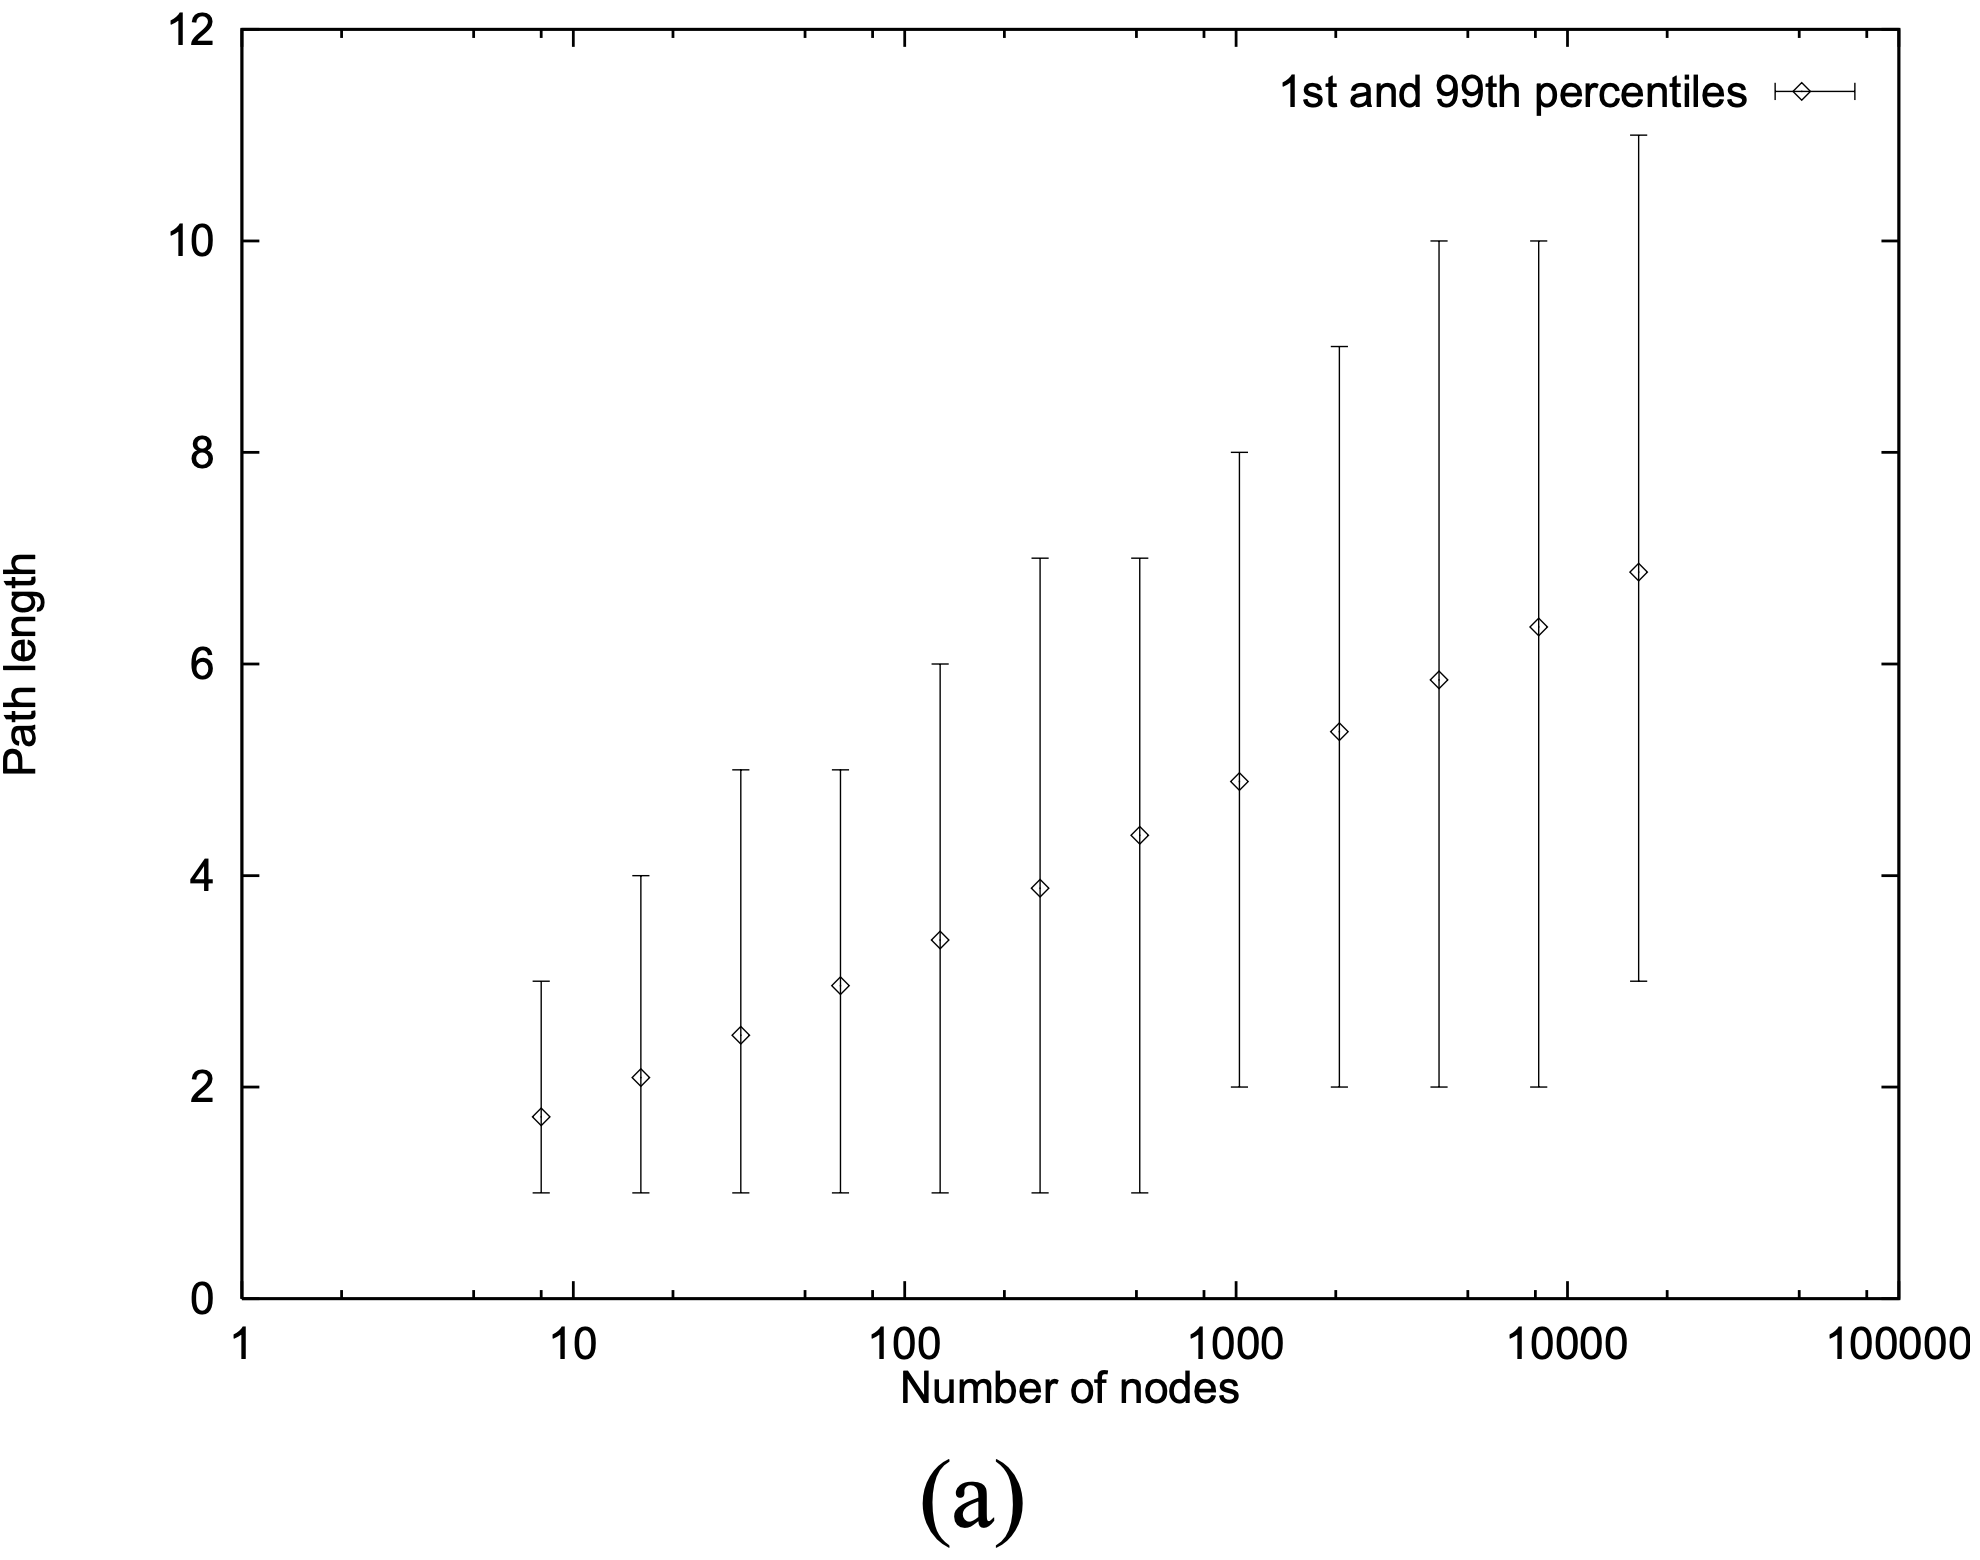
\includegraphics[width=0.8\textwidth]{gfx/chord-performance.png}
    \caption{Chord performance \cite{chord}, Figure 10 (a)}
    \label{fig:chord-performance}
\end{figure}

\subsubsection{Pastry}

Pastry \cite{pastry} is a DHT that uses a ring topology.
It provides only the routing algorithm, and implements no application-level functionality.
It uses a $2^{128}$ keyspace, and nodes' IDs are either a cryptographic hash
of their IP address or their public key.
Pastry uses a more complex routing algorithm than Chord, by making use of a table with
neighbors that share a common prefix with the node.
The routing algorithm utilizes prefix routing using the table.
It also uses locality based on IP routing hops in order to optimize the routing and speed.
A difference from Chord is how Pastry deals with node failures lazily.
This means that when a node fails, the network will remove it from the routing tables of other nodes
only when they try to access it.
The paper explores a network with 5000 nodes where 10\% (500) of the nodes fail.
To repair such a failure 200,000 queries were required.
Pastry does not address replication and recovery of data.

\subsubsection{PAST}

PAST \cite{past} is a storage solution implemented on top of Pastry.
A file is stored under a unique fieldID (key),
which is generated at the time of insertion into the network.
PAST does not support deletion, it provides a reclaim operation, which marks a file as
"can be deleted", but does not force its deletion.
In terms of security PAST assumes most nodes are honest and does not provide much protection against
malicious nodes.
It does address data integrity by using a cryptographic hash of the file,
which is used to verify the integrity upon retrieval.
The paper also briefly mentions random audits to see if the data is still available,
but provides no details on how this would be implemented or what the effectiveness is.
The integrity checks are done by utilizing a new concept that the paper introduces --- smart cards.
Smart cards have 2 parts --- a private key, used to sign data and contracts and a balance section.
The balance indicates how much data this peer is storing in the network versus how much it is storing locally.
This balance is used to disallow freeloaders and deal with malicious nodes trying to flood the
network with fake data.

\subsubsection{Kademlia}

Kademlia \cite{kademlia} is one of the most popular structured DHTs.
It uses a hypercube topology (a binary tree organizing nodes based on their XOR distance)
and is used as the basis for many other DHTs.
Kademlia uses a $2^{160}$ keyspace, which is navigated using a XOR metric.
Replication is optional and is achieved by storing the file on the $k$ closest nodes to the key of the file.
The keys are usually hashes of the file contents.
This enables a basic form of data integrity, as the file can be verified by comparing its hash to the key.
However, this does not allow users to choose the key of the file.
Kademlia does not provide anonymity to the users, as the network operates based on node IDs,
which are public and can potentially be traced back to individual users.
Stored data in the network needs to be republished every 1 hour to ensure that the file is still available,
as records expire after 24 hours.
The base Kademlia does not employ any security mechanisms, unless accidental such.
For example, Eclipse attacks and Churn attacks are mitigated by
the fact that the network favors longer-lived nodes over new ones.
The network uses the republishing mechanism to ensure that the data remains available when nodes
leave or join the network.
The fault tolerance relies on the above mechanism,
as well as the fact that the network favors longer-lived nodes over new ones.
Queries in Kademlia take $O(\log n)$ hops to reach the correct node, where $n$ is the number of nodes in the network.

\subsubsection{S/Kademlia}

S/Kademlia \cite{skademlia} is a secure version of Kademlia.
It is the security extension of Kademlia and addresses the main attacks on decentralized networks.

To address Sybil attacks S/Kademlia employs a proof-of-work mechanism --- a cryptographic puzzle that
the joining node must solve.
It also proposes a solution for adversarial routing by sending multiple queries to different parts
of the network and comparing the results.
The routing algorithm is also improved to be more resistant to adversarial routing
by running multiple disjoint queries in parallel and comparing the results (Figure \ref{fig:skademlia-eval}).
The paper does not cover data storage attacks.
DDoS attacks are not covered by the paper.
These are usually attempted to be solved by rate limiting, throttling, and traffic filtering,
however there are no guarantees that these will work against a sufficiently large attack.

\begin{figure}
    \centering
    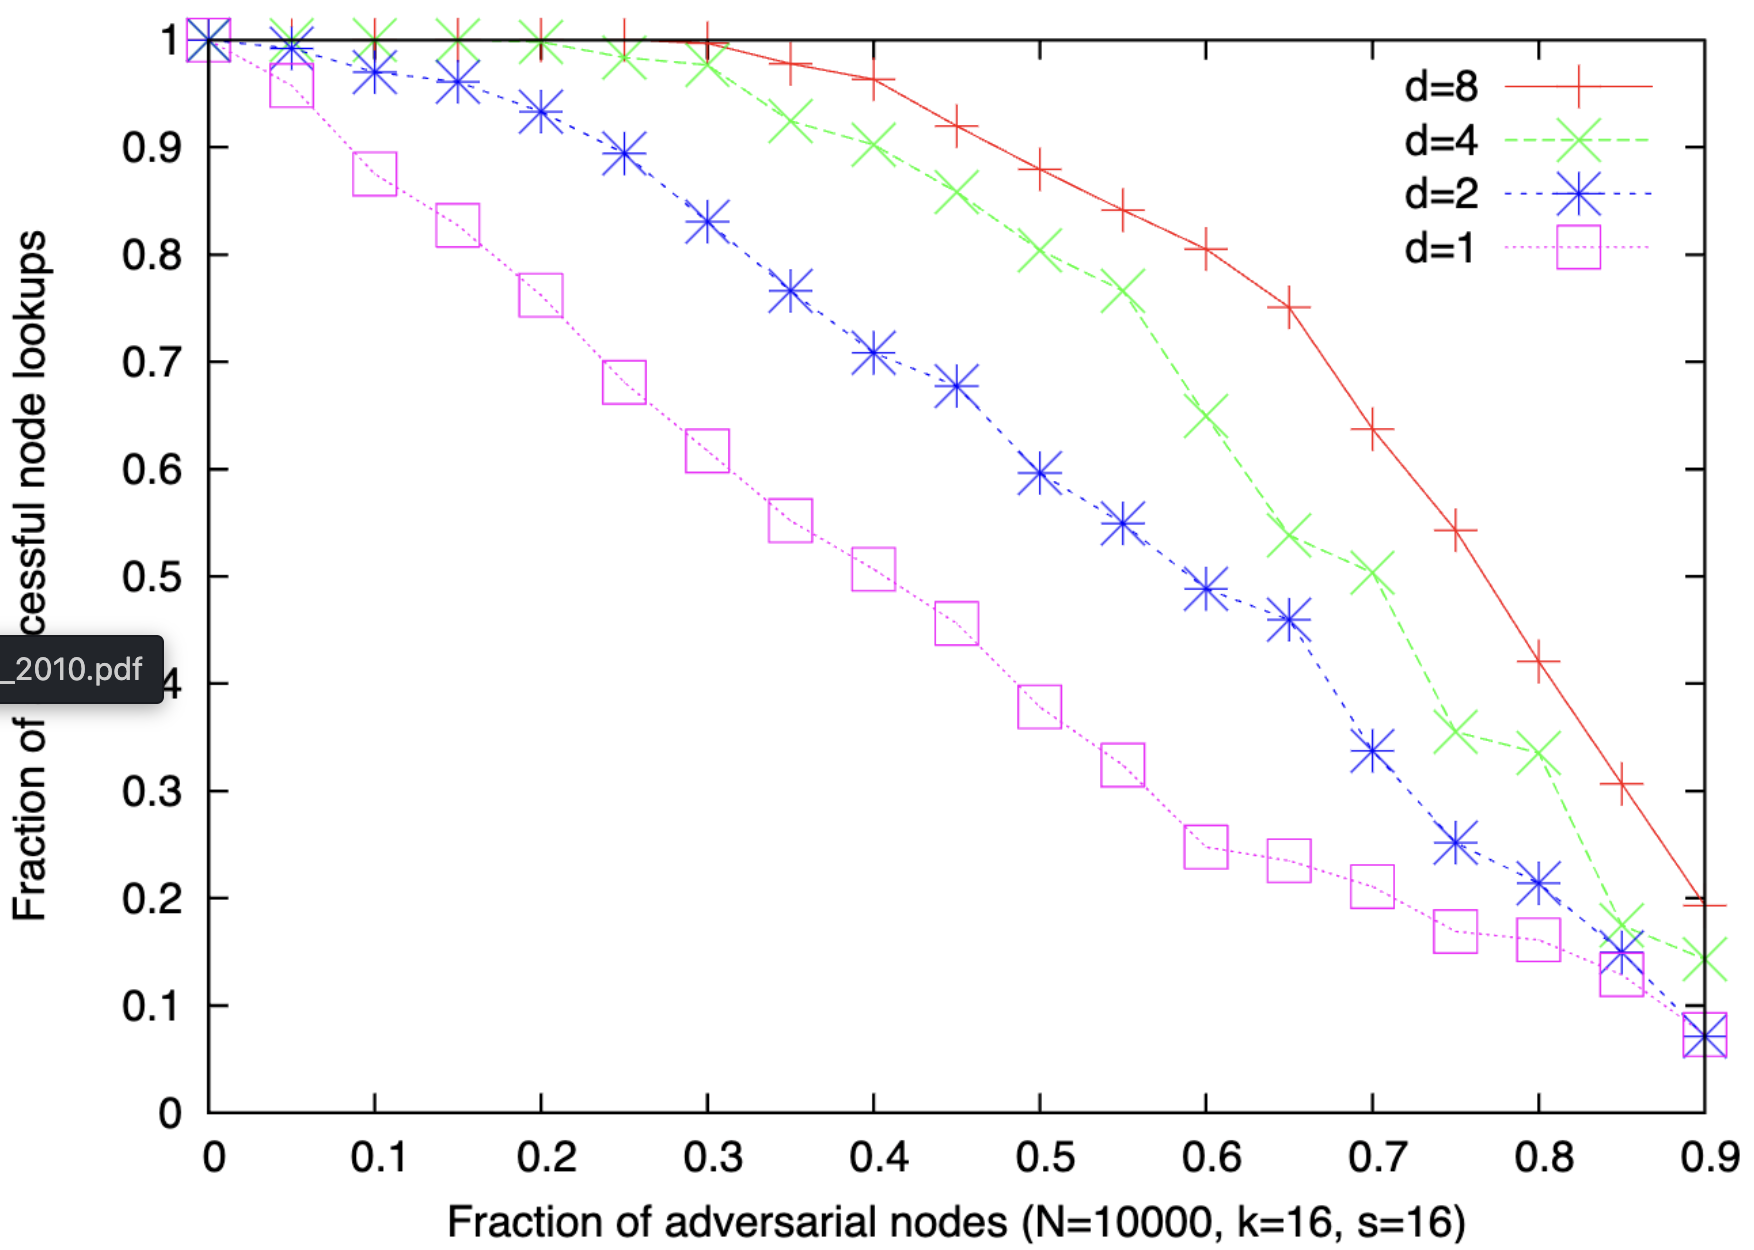
\includegraphics[width=0.8\textwidth]{gfx/skademlia-eval.png}
    \caption{S/Kademlia node lookup success with $d$ disjoint paths and $k$ neighbor bucket size \cite{skademlia}, Figure 4 (a)}
    \label{fig:skademlia-eval}
\end{figure}

\subsubsection{Freenet}

Freenet \cite{freenet} is a DHT that focuses heavily on anonymity.
Another classic example of a network that provides no guarantees about the longevity of the data.
It uses replication by aggressive caching during retrieval to hide where the data is stored originally.
It also anonymizes the queries and the responses by using onion routing-style techniques.
However, this means that the network heavily relies on peers being honest.
The keyspace is $2^{160}$.
The node ID is the XOR of the seeds of a number of nodes.
Which means that the ID will be truly random, however it might allow a form of DoS attack
where malicious nodes join the network in bulk, flooding it with traffic.
Files are stored under hashes of the public key of a user-chosen string (description).
The private key is used to sign the file as a basic form of data integrity.
This enables dictionary attacks and key-squatting, which is a natural downside of a system
that focuses on anonymity.
Interesting new concept is the support of pointers, which allow the user to store a file under a key,
and then store other keys that simple point to the same file.
It uses a custom routing algorithm, whose performance can be seen in Figure \ref{fig:freenet-algo}.

\begin{figure}
    \centering
    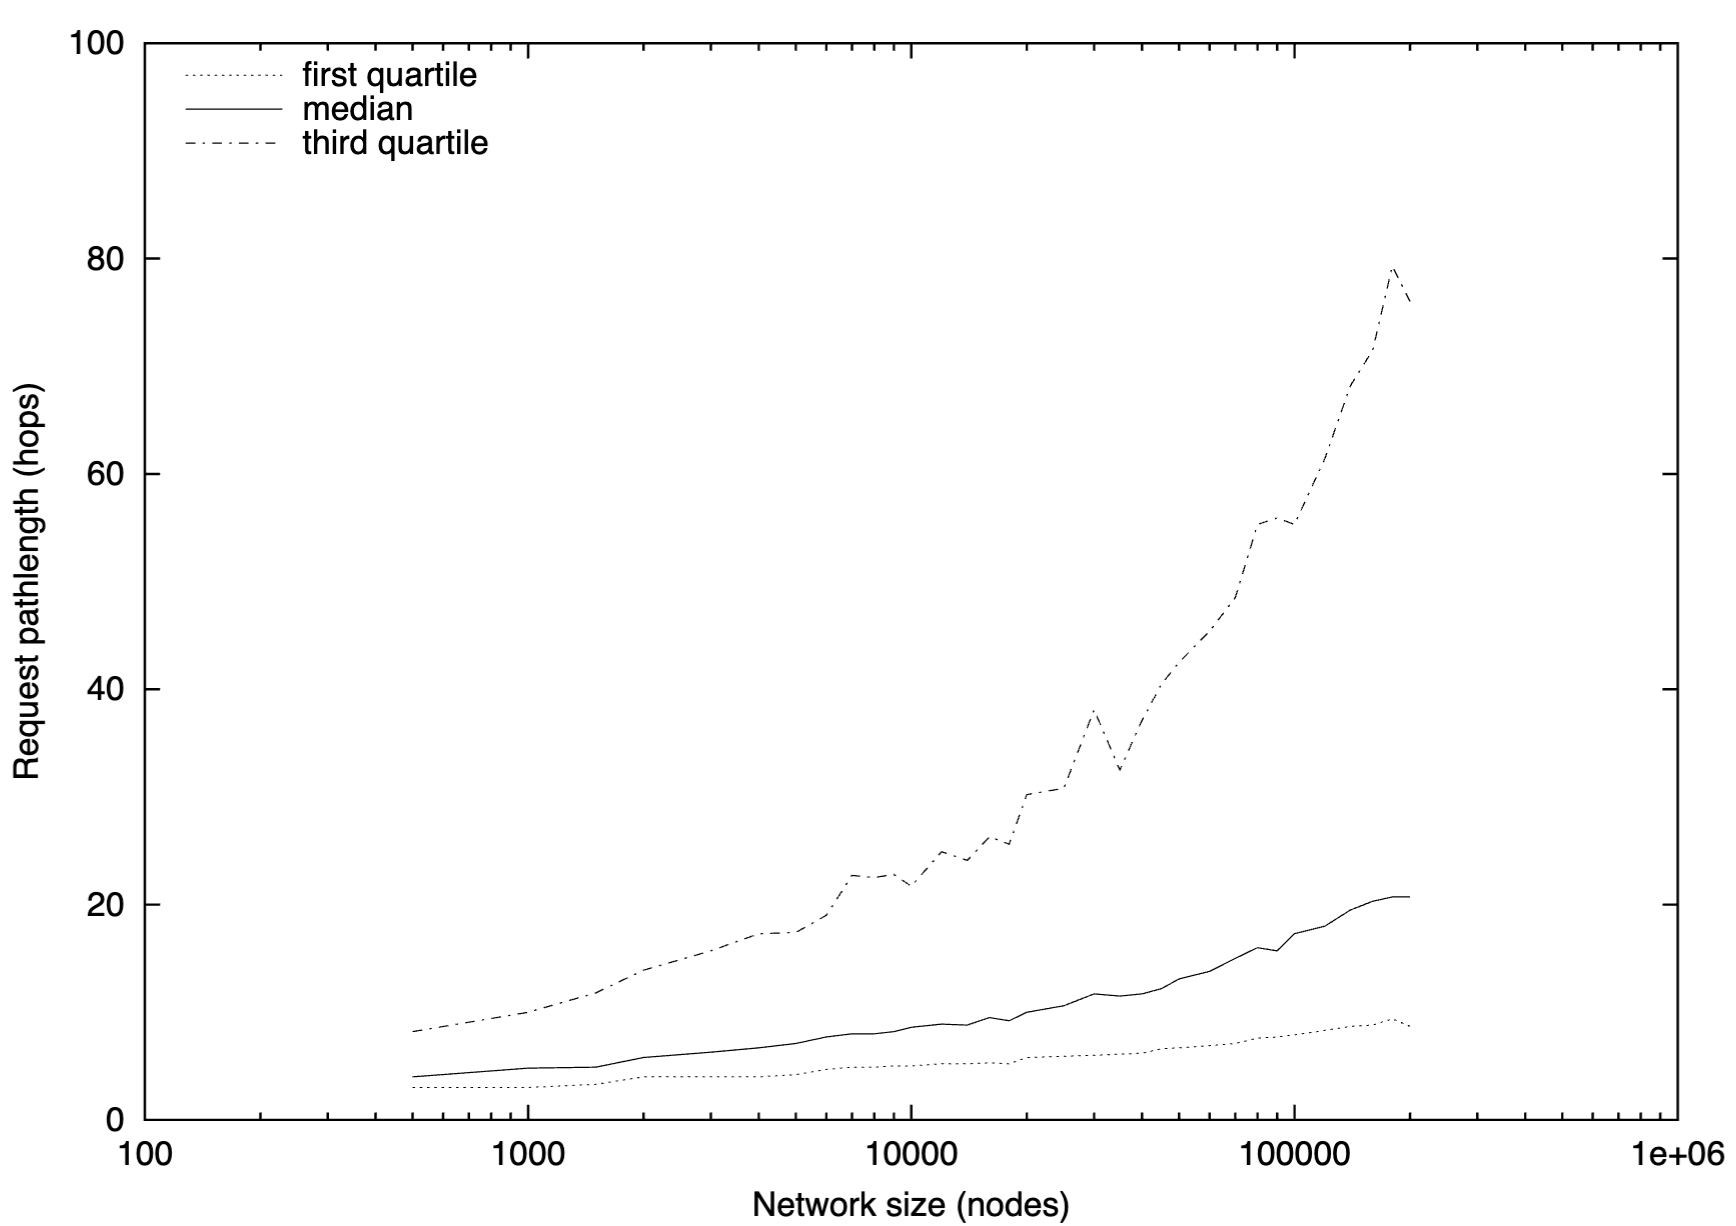
\includegraphics[width=0.8\textwidth]{gfx/freenet-algo.png}
    \caption{Freenet uses a hybrid routing algorithm that is between structured and unstructured,
        which results in higher number of hops, and hence lower performance \cite{freenet}, Figure 3}
    \label{fig:freenet-algo}
\end{figure}

\subsection{Large scale storage networks}

\subsubsection{IPFS (InterPlanetary File System)}
IPFS is a DHT that provides human-friendly names for files.
However, if a user wants their files to be verifiable, they can create a personal namespace (a subdirectory),
which is their public key, and store files under it.
In this case the name is no longer human-friendly, but the files are verifiable.
Human-friendly names have a downside that they could be subject to a dictionary attack and
squatting --- where a malicious user could register a name similar to a popular one and
serve malicious content.
IPFS makes use of Merkle DAGs in order to uniquely identify files and to ensure tamper resistance,
as files can be verified by comparing their hash to its checksum.
The system doesn't provide persistence guarantees.
It relies on popular files being requested often enough, so they can be cached by different nodes.

IPFS \cite{ipfs} uses the BitSwap protocol, which allows peers to exchange partial blocks of data,
similarly to BitTorrent.
Peers can barter for the blocks they need, or choose to store rare pieces of data to increase their reputation.
The authors hint at using a ledger to keep track of the reputation (currency) of the peers,
but leave it as future work.
The BitSwap protocol borrows a lot from BitTorrent, and acknowledges that there are exploits such as
BitTyrant \cite{bittorrentexploits} and BitThief \cite{bittorrentexploits}
that can be used to exploit the protocol.
Preventing these exploits however are left as future work.

\subsubsection{OceanStore}

OceanStore \cite{oceanstore} another storage network aiming at scaling to serve trillions of files.
To achieve this, the paper proposes a two-tiered query algorithm.
First, a probabilistic fast query is used, based on bloom filters, and if it fails,
a slower hierarchy based query is issued.
In terms of security the paper discusses only DDoS attacks.
It proposes hashing the file ID with multiple salts to generate different keys,
which are then used to store the file on different nodes.
This distributes the file across the network differently than sequential replication.
To ensure data integrity OceanStore splits the files into chunks and stores them on different nodes.
It also uses erasure codes so that the file can be restored from any $k$ out of $n$ chunks.
Another network that is very similar and dives deeper into erasure codes is Tahoe \cite{tahoe}.

\subsection{Blockchain-based networks}

\subsubsection{Sia}
Sia \cite{sia} is a blockchain-based storage network.
The network stores storage contracts in a blockchain, while the data itself is stored by the peers.
Sia aknowledges the need for auditing and that it is better for the network itself to audit the files, instead of requiring the clients to do so.
In terms of replication, the network has no in-built such --- it proposes the users to upload the same file multiple times.
When creating a contract the client specifies how often the audits happen, as well as the price paid out for a successful audit.
Contracts also have an upper limit of failed audits, after which the contract is terminated.
Sia utilizes merkle trees to perform the audits, which results are then sent to the blockckain so they can be verified by anyone.
The paper also proposes clients to use erasure codes, but they do not come built-in.
To prevent Sybil attacks, the network requires peers to lock in coins when advertising themselves as available to store data.
This way, it becomes expensive for peers to join en masse and it requires them to make a commitment to the network.
Balancing rewards and punishments is left to the client to decide, as they get to propse the contract as well as choose which peer to store it at.
While the paper proposes a lot of innovative ideas, it does not fully explore most of them and it doesn't evaluate them under what paramemters they make sense.

\subsubsection{Filecoin}

Filecoin \cite{filecoin} is another blockchain-based storage network,
which is a direct upgrade of Sia and works on top of IPFS.
Filecoin is described as a decentralized storage network that turns cloud storage into an algorithmic market.
It also introduces its own cryptocurrency, which powers the transactions in the market.
Coins are earned by storage nodes, that store the data, and by retrieval nodes, that serve the data,
and they are paid by the clients.
The way tokens are awarded to the nodes is in micropayments done by the client after a successful audit/retreival.
The paper defines Data Integrity as the ability to prove that retrieved data is untampered with,
and Retrievability as the ability to prove that the data is still available.
There is a catch in the definition of Retrievability --- it works under the assumption that the peers
follow the protocol.
It does not address the case where the peers are malicious and stop serving the data.
This is the first instance where Proof of Retrievability is mentioned in the context of decentralized storage,
however the paper does not use the modern PoR protocols, and assumes PoR is probabilistic and proves
that a server is storing some part of the data, but not necessarily all of it.
For the audits Filecoin uses a custom protocol named Proof of Replication, which is a variant of PoR.
In simple words, Proof of Replication works by storing each replica of a file encrypted with a different key,
which makes each file different, it then issues cryptographic challenges as audits.
To build on top of it also makes use of Proof of Spacetime, which is a protocol that proves that a node
has been storing data for a certain amount of time.

\subsection{Other networks}

\subsubsection{ARA}

ARA is not a storage network, but proposes ways to deal with free-riding in peer-to-peer networks.
The paper assumes a specific kind of malicious peer, that is selfish, i.e., does not want to contribute their resources to the system.
The paper proposes a decentralized economy system, similar to performing micro-paymets to a server.
The introduction of an economy means the possible subset of attacks is mainly related to disrupting said economy.
To deal with these attacks the paper proposes audits on the transactions and the credits of each peer.
The audits rely on cryptographic signatures and at least one non-malicious peer that can perform the audit.
The audit is essentially checking the claim of the malicious peer for how much data they store versus how much has been recorded that they should store in the system's ledger.
The paper does not cover content cheating (file integrity) as they argue it is not feasible without human intervention.

\subsection{Summary}

Decentralized networks have evolved over the years with each new network building on top of the previous ones,
by adding a new feature such as anonymity, security, a new routing algorithm, or introduction of a new technology
such as blockchain.
With networks becoming so complex, they tend to focus on a particular problem,
for example anonymity or security.
This is also due to the fact that the solutions to some problems are mutually exclusive,
for example, anonymity and security.
The tendency in the security direction is to address as many attacks as possible,
with the latest networks making use of ledger stores and reputation systems.

\section{Proof of Retrievability}

Proof of Retrievability (PoR) \cite{porfirst} is a cryptographic protocol that
allows a client to verify that a server is storing a file.
The server is challenged to prove that it is storing the file, and the client
can verify the proof.
PoR protocols are designed to be used to check the integrity of the data stored by cloud providers mostly.

There are 2 state of the art PoR techniques:
\begin{itemize}
    \item From 2020, "Dynamic proofs of retrievability with low server storage" \cite{poralgebra} —
        based on an algebraic approach, involving matrix multiplication.
    \item From 2022, "Efficient Dynamic Proof of Retrievability for Cold Storage" \cite{pormerkle} —
        based on a purely cryptographic approach with Merkle trees.
\end{itemize}

"Dynamic proofs of retrievability with low server storage" introduces a protocol, which 
requires $N + O(N/\log N)$ server storage, where $N$ is the size of the file.
The protocol is dynamic, meaning that the client can update the file and the server can update the proof.
This feature could be important for some decentralized storage systems, which split the files into chunks and
store them on different nodes.
However, splitting the file between multiple nodes will make the audit process more complex and time-consuming.
The client stores $O(\sqrt{N})$ data.
This is still not perfect, as in a decentralized storage system each node is a client, hence knows the secret.
This can be addressed with the last contribution of the paper --- public verifiability.
Public verifiability is a variant of the proposed protocol that allows any untrusted third party
to conduct audits without a shared secret.

"Efficient Dynamic Proof of Retrievability for Cold Storage" makes improvements to the bandwidth and
client storage requirements of the previous protocol.
The audit proof is $O(1)$ --- a fixed number of group elements sent from the server to the client.
Client storage is reduced to a single master key, the size of the security parameter,
which is again constant.
Public verifiability is also possible with logarithmic overhead.

Proofs of Retrievability are an important instrument to ensure integrity in decentralized storage.
